\documentclass[11pt, a4paper]{article}

\usepackage[utf8]{inputenc}
\usepackage[italian, english]{babel}
\usepackage[pages=some]{background}
\usepackage{hyperref}
\usepackage{float}
\usepackage{amsmath}

\graphicspath{ {./img/} }
\backgroundsetup{
	firstpage = {true},
	placement = {center},
	position = current page.center,
	contents = {
\includegraphics[scale=0.07]{unipd}},
	angle = {0},
	opacity = {0.03}
}
\hypersetup{
	colorlinks=true,      
	urlcolor=blue,
	linkcolor=black
}

\newcommand{\image}[3]{
	\begin{figure}%[H]
		\centering
		\includegraphics[width=0.9\textwidth]{#1}
		\caption{#2.}
		\label{#3}
	\end{figure}
}

\title{Vision and Cognitive Services\\
\large Video Frame Interpolation via Adaptive Separable Convolution}
\author{Filippo Visentin (matricola)\\
Nicola Carlesso (1237782)}
\date{a.a. 2020/2021}

\begin{document}
	\pagenumbering{gobble}
	\maketitle
	\clearpage
	
	\tableofcontents
	\clearpage
	\pagenumbering{arabic}
	
	\section{Introduction}
	Our work is related on the video frame interpolation problem. In particular we look at work in \cite{mainpaper}; when we talk about ``our network'', we refer to a modified version of the network in \cite{mainpaper}.\\
	The video frame interpolation problem consists of recreating the frame between two input frames in a video. This problem allows either to obtain a higher quality video, in terms of frames per second, or a more defined slow motion, or a super slow motion.\\
	The main challenge of this problem is to get an output frame with defined shapes, because the network tends to give in output a blurred frame, and recreate a good frame in case of the two input frames are quite different.\\
	Our network has a decoder-encoder architecture, used mainly to recreate fake example from a dataset, as in our case study. The network doesn't create directly the interpolated frame, but gives in output an ad hoc couple of kernels (separable kernels) for each input frame. As last step we apply the convolutional operation with output kernels and input frames to get the output frame. 
	
	\section{Related work}
	Other approaches to resolve this problem are with the optical flow technique \cite{optical_flow}, where the network learns movements of figures in the frame and predicts those immediately following. This technique requires two main steps: first estimate optical flow between input frames and then synthesize an intermediate frame guided by motion; our approach requires instead a single convolution process.\\
	The work we rely on is a continuation of another work in \cite{previous_work} that use our same network structure with one, mainly difference: in our network we obtain two separable kernels for each input frame, a column and a row vector, in \cite{previous_work} the network gives in output one ``standard'' kernel (a square matrix) for each input frame. This difference gives a big improvement in terms of memory and computational time. Because in our case the network gives only a column and a row vector, instead of a matrix, in fact the usage of memory went from 26GB to 1.27GB.  In this way, an $n\times n$ convolution kernel can be encoded using only $2n$ variables.\\
	Another improvement is the sharpness and quality of output frames.
	
	\section{Dataset}
	Fortunately, for the video frame interpolation problem, its easy to create a large dataset without looking online.\\
	We just have to take a video and extract a triplet of close frames. The input are the first and last frame of triplet, and the label is the second frame. Its important consider two factors:
	\begin{itemize}
		\item all frames in triplet must be enough different, otherwise the example will be useless for the learning phase;
		\item all frames in triplet don't must be too much different. For example, in the case of in the middle of triplet a change of scene occurs. 
	\end{itemize}
	Therefore, we analysed the difference of image histograms of triplet's frames to have the magnitude of motion and then we compared them by taking the norm of the difference vector, setting a lower and an upper bound.\\
	Another important hyper-parameter used to create the database is the number of frames between elements of the triplet. In this way we have examples that can show more os less movement, this to test the strength of network.\\
	To create our dataset we use \href{https://www.crcv.ucf.edu/data/UCF101.php}{UCF-101} and the Python script\\ \texttt{dataset/create\_dataset.py}.\\
	With all dataset UCF-101, we can get about 500'000 examples. Unfortunately, already with 150'000 examples and a \textit{batch size} of 32 examples, an epoch requires about 1 hour of time, so we used for our experiment a dataset of 50'000 examples (we note that using 50'000 or 75'000 examples, the results doesn't change too much).
	 
	%% iniziare avendo scritto circa 2 pagine
	\section{Method} %% quasi 2 pagine
	Our structure of the CNN used is based on that of \cite{mainpaper}, showed in Figure~\ref{original-net}, with some changes. At the core there is a encoding phase with 6 steps of 3-stack of convolutional layers, separated by pooling layers. The decoding phase is the reverse of previous, with a bilinear upscaling. The upscaling reintroduces feature maps from the encoding layer, in order to facilitate the decoding. As output of the net we expect a couple of separable kernels for each pixel, used to combine pixels from the 2 input frames to obtain each new pixel of the interpolated frame. In the network is used the skip connection technique to let the expanding layers incorporate features from the contracting part of the neural network.\\
	If we call $I_1$ and $I_2$ two input frames and $\hat{I}$ the interpolated frame, to compute each output pixel $(x,y)$, the final stage applies at each input frame a convolutional operation between every output kernel and patches centred in $(x,y)$.\\
	As we ca see in Figure~\ref{original-net}, if we consider inputs like a matrix $128\times128$ and we set the size of separable kernels as $51\times1$, the output of network (with batch size of 1) are four matrices $128\times128\times51$: $k_{1,h}$, $k_{1,v}$, $k_{2,h}$, $k_{2,v}$; $k_{n,s}(x,y)$ is a vector $51\times1$.\\
	For the last step, given the output of network, we call $K_n(x,y) = k_{n,h}(x,y) \cdot k_{n,v}(x,y)$, a matrix $51\times51$ and the input patch centred in $(x,y)$ of \textit{n-th} input frame $P_n(x,y)$, always a matrix $51\times51$.\\
	Each output pixel $\hat{I}(x,y)$ is calculate using the Equation~\ref{eq} (``$*$'' represents the point-wise multiplication and the sum of matrix's values). We can observe that when we make this operation for each pixel, we obtain the convolutional operation. 
	
	\begin{equation}
		\hat{I}(x,y) = K_1(x,y) * P_1(x,y) + K_2(x,y) * P_2(x,y)
		\label{eq}
	\end{equation}
	
	\image{net_structure}{Structure of original convolutional network. Note that $\dot{*}$ denotes a local convolution.}{original-net}

	\section{Experiment} %% quasi 2 pagine
	In order to improve the performance of the network we explored many solutions, some of which not useful and some more interesting.\\
	Initially we maintain the original structure of the network, trying to change some parameters, but without significantly improvements. We tried to:
	\begin{itemize}
		\item \textbf{Normalization:} we applied the normalization to the input images, calculating mean and variance, and for the last step the denormalization, in order to obtain a better learning. That has proven ineffective, as dataset were already nearly normalized by their own;
		\item \textbf{Dropout:} the goal was improve performances and speed of network, but we don't observe noticeable difference in accuracy or computing time. Dropout helps to generalize what network is learning. We assume that this encoding-decoding architecture can generalize well enough that it doesn't need to dropout; 
		\item \textbf{Optimizer:} in CNN the mostly used optimization algorithm is Adam, so we use it for our experiments. We tested other optimization algorithms, like AdaMax or SDG, but without improvements.
	\end{itemize}
	Maintaining Adam as optimizer, without normalization and dropout, we tried to modify the structure of network and the loss function, to compare the results in \cite{mainpaper} that similarly tried the network with different loss functions.\\
	We applied two main changes to the network, getting interesting improvement:
	\begin{itemize}
		\item We remove from every coding and decoding step a convolutional layer, transforming it from 3-stack to 2-stack convolutional layers. In this way the time per epoch reduces by about 30\% and the network trains faster without the risk of under fitting;
		\item In the last step, when we apply the output network to the Equation~\ref{eq}, we add two additional convolution layers to see if kernels with a further convolutional operation can return better results. 
	\end{itemize}
	Finally, we note that the network is able to overfit (if given enough epochs) even with large datasets, but 15-20 epochs are enough to avoid it.
	
	\subsection{Loss functions}
	In \cite{mainpaper} the authors used two loss function: MSE and a perceptual loss, that is usually based on high-level features of	images. They empirically found that the feature reconstruction loss based on the \texttt{relu4\_4}\footnote{\label{vgg-structure}To see the structure of VGG-19 with name of layer, visit \url{https://it.mathworks.com/help/deeplearning/ref/vgg19.html}} layer of the VGG-19 network produces good results for the frame interpolation task.\\
	Following the idea of using feature maps to create a loss function, we decided to try some handcrafted filters, therefore we used four different loss functions:
	\begin{itemize}
		\item \textbf{MSE}
		\item \textbf{VGG19-44}: we used the pretrained VGG-19 weights until layer \texttt{relu4\_4}. This because a one comparison of pixels focuses on really fine details and losses on the overall (local) appearance of the image. VGG-19 extracts features, focusing more on discriminative information (for classification) than e.g. noise;
		\item \textbf{VGG19-21}: we found that taking an earlier layer of the VGG-19 network, the \texttt{relu2\_1}\footref{vgg-structure} gives a more interesting loss. At late layers the loss focuses on overall shapes, in this way our network matches harder the shape instead of its position on figures;
		\item \textbf{FixKernel}: we created a mini network with two convolutional layers with vertical and horizontal Sobel filters and then me compute MSE with the output.
	\end{itemize}
	 
	\image{mse_loss2}{The Mean square error loss is blurry}{loss-mse}
	\image{vgg16_relu4_4_loss2}{Taking the VGG-19 at a late layer makes our network choose between one of the 2 inputs}{loss-vgg19-44}
	\image{vgg16_relu2_1_loss2}{Taking it at a early layer gives some sort of trade off}{loss-vgg19-21}

	\begin{figure}
		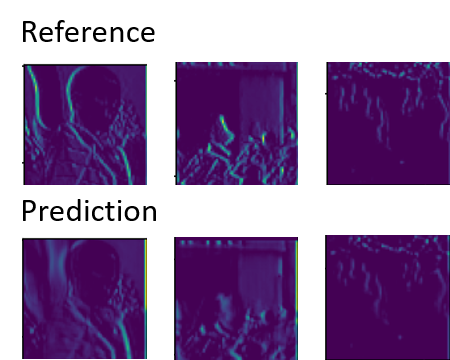
\includegraphics[width=.5\textwidth]{map_sobel}
		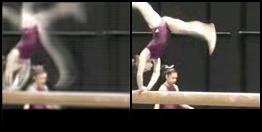
\includegraphics[width=.3\textheight]{sobel}
		\caption{Using a \textbf{sobel} filter we try to focus on edges, so output images remain defined. Here we show also the feature maps obtained}
		\label{feature-map}
	\end{figure}
	\begin{figure}
		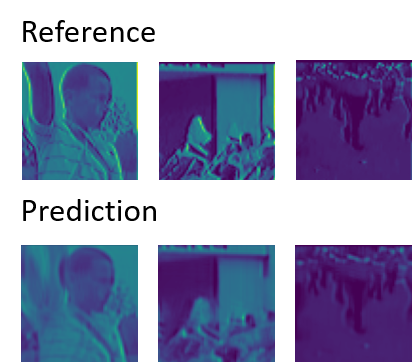
\includegraphics[width=0.3\textheight]{sobel_color_map}
		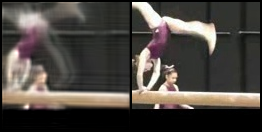
\includegraphics[width=0.3\textheight]{sobel_color}
		\caption{To avoid losing all the information on color, we modified the filter to also consider a bit the central pixel \textbf{color}}
		\label{color-feature-map}
	\end{figure}
	We decided to use the last one at the end as the use of VGG-19 makes the learning slower and also because it retains color information without loosing too much on definiteness.

	\subsection{Image refining layers}
	\subsection{Dvd Logo}
	%% vedere se impara la traslazione
	Testing our network with with VGG-19 filters, we saw that the interpolate frames tended to be identical to one of two input frames. To test if the network actually learns the movement of figures in an image, we tested the network with video that show a single object that make a translation (the simplest movement); like this \href{https://www.youtube.com/watch?v=5mGuCdlCcNM}{Youtube video}.\\
	As result, we see that if in the whole dataset we introduce some of these examples, network can effectively learns the movements of figures in the video. 
	
	\section{Conclusion}
	The video frame interpolation task can also helps for action recognition task in the pretrained phase, in the case of we want to see movements more detailed.
	
	\bibliographystyle{unsrt}
	\bibliography{bibliography}
	
\end{document}